\documentclass{article}
\usepackage[utf8]{inputenc}
\usepackage{polski}
\usepackage[polish]{babel}
\usepackage{bbm}
\usepackage{graphicx}
\usepackage{caption}
\usepackage{subcaption}
\usepackage{epstopdf}
\usepackage{amsmath}
\usepackage{amsthm}
\usepackage{hyperref}
\usepackage{url}
\usepackage{comment}
\newtheorem{defi}{Definicja}
\newtheorem{twr}{Twierdzenie}
\usepackage{listings}
\usepackage{float}
\usepackage{geometry}
 \geometry{
 a4paper,
 total={170mm,257mm},
 left=25mm,
 top=25mm,
 }

\author{Michał Martusewicz 282023}
\date{Wrocław, \today}
\title{\textbf{Model konceptualny bazy danych na Wielką Konferencję w (zapewne) Hotelu Hilberta}}

\begin{document}
\maketitle
\section{Diagram E-R}
\begin{figure}[H]
    \centering
	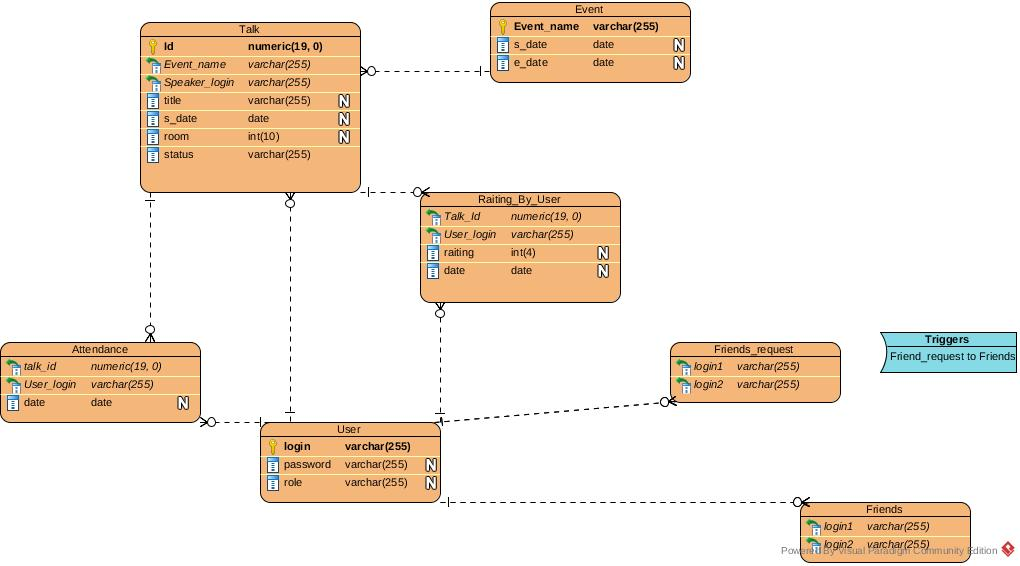
\includegraphics[width= 1 \textwidth]{Konferencja.jpg}
    \caption{Diagram E-R bazy danych na konferencję}
 	\label{diagram}
\end{figure}
\section{Więzy integralności i role}
Docelowo w bazie danych zamierzam mieć tylko jedną rolę - API, z pełnymi uprawnieniami administratora.
W bazie będzie jeden wyzwalacz, który przed wpisem do tabeli Friend\_request krotki (login1, login2) sprawdzi, czy nie ma już w niej (login2,login1). Jeżeli jest, to usunie ją z tej tabeli i wpisze dwie krotki: (login1,login2) i (login2,login1) do tabeli Friends.\\
Zamierzam użyć dwóch dodatkowych typów danych:
\begin{enumerate}
\item Status: SET('P','W','R') - (P - Public, W - Waiting, R - Rejected)
\item Role: SET('U','A') - (U -  User, A - Admin)
\end{enumerate}
Nie przewiduję usuwania danych, ze względu na dodatkowe pole 'status' w tabeli "Talk".

\end{document}
